\documentclass[twoside]{book}

% Packages required by doxygen
\usepackage{fixltx2e}
\usepackage{calc}
\usepackage{doxygen}
\usepackage[export]{adjustbox} % also loads graphicx
\usepackage{graphicx}
\usepackage[utf8]{inputenc}
\usepackage{makeidx}
\usepackage{multicol}
\usepackage{multirow}
\PassOptionsToPackage{warn}{textcomp}
\usepackage{textcomp}
\usepackage[nointegrals]{wasysym}
\usepackage[table]{xcolor}

% Font selection
\usepackage[T1]{fontenc}
\usepackage[scaled=.90]{helvet}
\usepackage{courier}
\usepackage{amssymb}
\usepackage{sectsty}
\renewcommand{\familydefault}{\sfdefault}
\allsectionsfont{%
  \fontseries{bc}\selectfont%
  \color{darkgray}%
}
\renewcommand{\DoxyLabelFont}{%
  \fontseries{bc}\selectfont%
  \color{darkgray}%
}
\newcommand{\+}{\discretionary{\mbox{\scriptsize$\hookleftarrow$}}{}{}}

% Page & text layout
\usepackage{geometry}
\geometry{%
  a4paper,%
  top=2.5cm,%
  bottom=2.5cm,%
  left=2.5cm,%
  right=2.5cm%
}
\tolerance=750
\hfuzz=15pt
\hbadness=750
\setlength{\emergencystretch}{15pt}
\setlength{\parindent}{0cm}
\setlength{\parskip}{3ex plus 2ex minus 2ex}
\makeatletter
\renewcommand{\paragraph}{%
  \@startsection{paragraph}{4}{0ex}{-1.0ex}{1.0ex}{%
    \normalfont\normalsize\bfseries\SS@parafont%
  }%
}
\renewcommand{\subparagraph}{%
  \@startsection{subparagraph}{5}{0ex}{-1.0ex}{1.0ex}{%
    \normalfont\normalsize\bfseries\SS@subparafont%
  }%
}
\makeatother

% Headers & footers
\usepackage{fancyhdr}
\pagestyle{fancyplain}
\fancyhead[LE]{\fancyplain{}{\bfseries\thepage}}
\fancyhead[CE]{\fancyplain{}{}}
\fancyhead[RE]{\fancyplain{}{\bfseries\leftmark}}
\fancyhead[LO]{\fancyplain{}{\bfseries\rightmark}}
\fancyhead[CO]{\fancyplain{}{}}
\fancyhead[RO]{\fancyplain{}{\bfseries\thepage}}
\fancyfoot[LE]{\fancyplain{}{}}
\fancyfoot[CE]{\fancyplain{}{}}
\fancyfoot[RE]{\fancyplain{}{\bfseries\scriptsize Generated by Doxygen }}
\fancyfoot[LO]{\fancyplain{}{\bfseries\scriptsize Generated by Doxygen }}
\fancyfoot[CO]{\fancyplain{}{}}
\fancyfoot[RO]{\fancyplain{}{}}
\renewcommand{\footrulewidth}{0.4pt}
\renewcommand{\chaptermark}[1]{%
  \markboth{#1}{}%
}
\renewcommand{\sectionmark}[1]{%
  \markright{\thesection\ #1}%
}

% Indices & bibliography
\usepackage{natbib}
\usepackage[titles]{tocloft}
\setcounter{tocdepth}{3}
\setcounter{secnumdepth}{5}
\makeindex

% Hyperlinks (required, but should be loaded last)
\usepackage{ifpdf}
\ifpdf
  \usepackage[pdftex,pagebackref=true]{hyperref}
\else
  \usepackage[ps2pdf,pagebackref=true]{hyperref}
\fi
\hypersetup{%
  colorlinks=true,%
  linkcolor=blue,%
  citecolor=blue,%
  unicode%
}

% Custom commands
\newcommand{\clearemptydoublepage}{%
  \newpage{\pagestyle{empty}\cleardoublepage}%
}

\usepackage{caption}
\captionsetup{labelsep=space,justification=centering,font={bf},singlelinecheck=off,skip=4pt,position=top}

%===== C O N T E N T S =====

\begin{document}

% Titlepage & ToC
\hypersetup{pageanchor=false,
             bookmarksnumbered=true,
             pdfencoding=unicode
            }
\pagenumbering{roman}
\begin{titlepage}
\vspace*{7cm}
\begin{center}%
{\Large My Project }\\
\vspace*{1cm}
{\large Generated by Doxygen 1.8.11}\\
\end{center}
\end{titlepage}
\clearemptydoublepage
\tableofcontents
\clearemptydoublepage
\pagenumbering{arabic}
\hypersetup{pageanchor=true}

%--- Begin generated contents ---
\chapter{Hierarchical Index}
\section{Class Hierarchy}
This inheritance list is sorted roughly, but not completely, alphabetically\+:\begin{DoxyCompactList}
\item \contentsline{section}{Fruit}{\pageref{classFruit}}{}
\begin{DoxyCompactList}
\item \contentsline{section}{Apple}{\pageref{classApple}}{}
\item \contentsline{section}{Grape}{\pageref{classGrape}}{}
\item \contentsline{section}{Orange}{\pageref{classOrange}}{}
\end{DoxyCompactList}
\item \contentsline{section}{List}{\pageref{classList}}{}
\item \contentsline{section}{List\+:\+:Node}{\pageref{structList_1_1Node}}{}
\end{DoxyCompactList}

\chapter{Class Index}
\section{Class List}
Here are the classes, structs, unions and interfaces with brief descriptions\+:\begin{DoxyCompactList}
\item\contentsline{section}{\hyperlink{structnode}{node} }{\pageref{structnode}}{}
\item\contentsline{section}{\hyperlink{structnode1}{node1} }{\pageref{structnode1}}{}
\item\contentsline{section}{\hyperlink{structnode__info}{node\+\_\+info} }{\pageref{structnode__info}}{}
\end{DoxyCompactList}

\chapter{File Index}
\section{File List}
Here is a list of all files with brief descriptions\+:\begin{DoxyCompactList}
\item\contentsline{section}{\hyperlink{Lab1_8c}{Lab1.\+c} }{\pageref{Lab1_8c}}{}
\end{DoxyCompactList}

\chapter{Class Documentation}
\hypertarget{classBody}{}\section{Body Class Reference}
\label{classBody}\index{Body@{Body}}


Inheritance diagram for Body\+:
\nopagebreak
\begin{figure}[H]
\begin{center}
\leavevmode
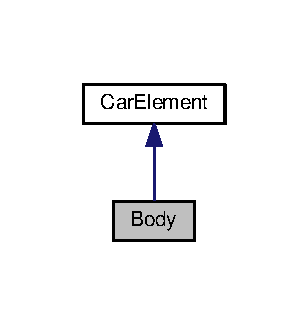
\includegraphics[width=148pt]{classBody__inherit__graph}
\end{center}
\end{figure}


Collaboration diagram for Body\+:
\nopagebreak
\begin{figure}[H]
\begin{center}
\leavevmode
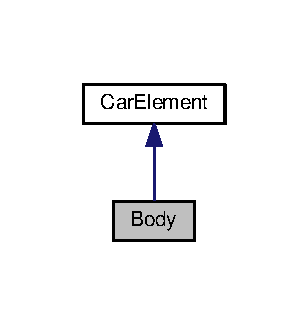
\includegraphics[width=148pt]{classBody__coll__graph}
\end{center}
\end{figure}
\subsection*{Public Member Functions}
\begin{DoxyCompactItemize}
\item 
void \hyperlink{classBody_a1a00b0272b72001a9c40303b719de342}{accept} (const \hyperlink{structCarElementVisitor}{Car\+Element\+Visitor} \&visitor)
\end{DoxyCompactItemize}


\subsection{Member Function Documentation}
\index{Body@{Body}!accept@{accept}}
\index{accept@{accept}!Body@{Body}}
\subsubsection[{\texorpdfstring{accept(const Car\+Element\+Visitor \&visitor)}{accept(const CarElementVisitor &visitor)}}]{\setlength{\rightskip}{0pt plus 5cm}void Body\+::accept (
\begin{DoxyParamCaption}
\item[{const {\bf Car\+Element\+Visitor} \&}]{visitor}
\end{DoxyParamCaption}
)\hspace{0.3cm}{\ttfamily [inline]}, {\ttfamily [virtual]}}\hypertarget{classBody_a1a00b0272b72001a9c40303b719de342}{}\label{classBody_a1a00b0272b72001a9c40303b719de342}


Implements \hyperlink{structCarElement_a9cac92d2d59d9a0318600e608bbbdfd5}{Car\+Element}.


\begin{DoxyCode}
65   \{
66     visitor.\hyperlink{structCarElementVisitor_aba7f494a9b736bcb002176ec922890e4}{visit}(*\textcolor{keyword}{this});
67   \}
\end{DoxyCode}


Here is the call graph for this function\+:
\nopagebreak
\begin{figure}[H]
\begin{center}
\leavevmode
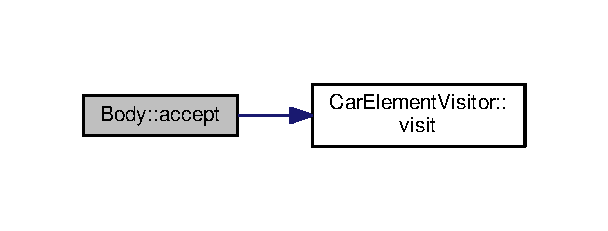
\includegraphics[width=292pt]{classBody_a1a00b0272b72001a9c40303b719de342_cgraph}
\end{center}
\end{figure}




The documentation for this class was generated from the following file\+:\begin{DoxyCompactItemize}
\item 
\hyperlink{Visitor_8cpp}{Visitor.\+cpp}\end{DoxyCompactItemize}

\hypertarget{classCar}{}\section{Car Class Reference}
\label{classCar}\index{Car@{Car}}


Inheritance diagram for Car\+:
\nopagebreak
\begin{figure}[H]
\begin{center}
\leavevmode
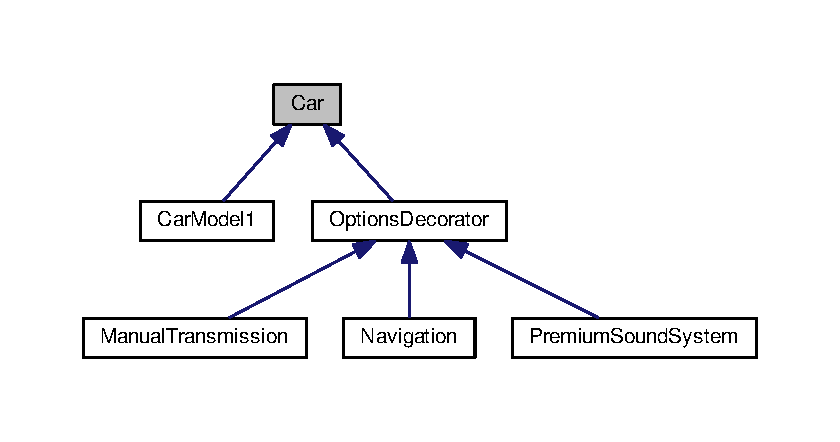
\includegraphics[width=350pt]{classCar__inherit__graph}
\end{center}
\end{figure}
\subsection*{Public Member Functions}
\begin{DoxyCompactItemize}
\item 
\hyperlink{classCar_a1c803f7c5038d3e31b368b0d0a35493c}{Car} ()
\item 
virtual string \hyperlink{classCar_a0d2f99b108e72e2a44360b38f16bbb46}{get\+Description} ()
\item 
virtual double \hyperlink{classCar_a7498766d25f7d4f15272f8055dd698f4}{get\+Cost} ()=0
\item 
virtual \hyperlink{classCar_a7f5f88d8a933b9de494e6beb818003f1}{$\sim$\+Car} ()
\end{DoxyCompactItemize}
\subsection*{Protected Attributes}
\begin{DoxyCompactItemize}
\item 
string \hyperlink{classCar_a2df6abd440445c77b48a45493245bb8e}{\+\_\+str}
\end{DoxyCompactItemize}


\subsection{Constructor \& Destructor Documentation}
\index{Car@{Car}!Car@{Car}}
\index{Car@{Car}!Car@{Car}}
\subsubsection[{\texorpdfstring{Car()}{Car()}}]{\setlength{\rightskip}{0pt plus 5cm}Car\+::\+Car (
\begin{DoxyParamCaption}
{}
\end{DoxyParamCaption}
)\hspace{0.3cm}{\ttfamily [inline]}}\hypertarget{classCar_a1c803f7c5038d3e31b368b0d0a35493c}{}\label{classCar_a1c803f7c5038d3e31b368b0d0a35493c}

\begin{DoxyCode}
11                 \{
12                         \hyperlink{classCar_a2df6abd440445c77b48a45493245bb8e}{\_str} = \textcolor{stringliteral}{"Unknown Car"};
13                 \}
\end{DoxyCode}
\index{Car@{Car}!````~Car@{$\sim$\+Car}}
\index{````~Car@{$\sim$\+Car}!Car@{Car}}
\subsubsection[{\texorpdfstring{$\sim$\+Car()}{~Car()}}]{\setlength{\rightskip}{0pt plus 5cm}virtual Car\+::$\sim$\+Car (
\begin{DoxyParamCaption}
{}
\end{DoxyParamCaption}
)\hspace{0.3cm}{\ttfamily [inline]}, {\ttfamily [virtual]}}\hypertarget{classCar_a7f5f88d8a933b9de494e6beb818003f1}{}\label{classCar_a7f5f88d8a933b9de494e6beb818003f1}

\begin{DoxyCode}
23                 \{
24                         cout << \textcolor{stringliteral}{"~Car()\(\backslash\)n"};
25                 \}
\end{DoxyCode}


\subsection{Member Function Documentation}
\index{Car@{Car}!get\+Cost@{get\+Cost}}
\index{get\+Cost@{get\+Cost}!Car@{Car}}
\subsubsection[{\texorpdfstring{get\+Cost()=0}{getCost()=0}}]{\setlength{\rightskip}{0pt plus 5cm}virtual double Car\+::get\+Cost (
\begin{DoxyParamCaption}
{}
\end{DoxyParamCaption}
)\hspace{0.3cm}{\ttfamily [pure virtual]}}\hypertarget{classCar_a7498766d25f7d4f15272f8055dd698f4}{}\label{classCar_a7498766d25f7d4f15272f8055dd698f4}


Implemented in \hyperlink{classManualTransmission_a33631e1b167a3aa7a2d86f5d8e2061bf}{Manual\+Transmission}, \hyperlink{classPremiumSoundSystem_ad14f7dae4adfb94572a80199174425af}{Premium\+Sound\+System}, \hyperlink{classNavigation_a2fedd3cf436e7487afc7a50d732d1054}{Navigation}, and \hyperlink{classCarModel1_aea624f25abb810c994dcd20f766418ed}{Car\+Model1}.

\index{Car@{Car}!get\+Description@{get\+Description}}
\index{get\+Description@{get\+Description}!Car@{Car}}
\subsubsection[{\texorpdfstring{get\+Description()}{getDescription()}}]{\setlength{\rightskip}{0pt plus 5cm}virtual string Car\+::get\+Description (
\begin{DoxyParamCaption}
{}
\end{DoxyParamCaption}
)\hspace{0.3cm}{\ttfamily [inline]}, {\ttfamily [virtual]}}\hypertarget{classCar_a0d2f99b108e72e2a44360b38f16bbb46}{}\label{classCar_a0d2f99b108e72e2a44360b38f16bbb46}


Reimplemented in \hyperlink{classManualTransmission_a3c5f0113936e6f8734a659ab8331a565}{Manual\+Transmission}, \hyperlink{classPremiumSoundSystem_a11267003bbf024bf19b811b0b28b22c1}{Premium\+Sound\+System}, \hyperlink{classNavigation_a2f7f7e9c43ecd76feabd46983b454e75}{Navigation}, and \hyperlink{classOptionsDecorator_a620341446534468345792530d454f76c}{Options\+Decorator}.


\begin{DoxyCode}
16                 \{       
17                         \textcolor{keywordflow}{return} \hyperlink{classCar_a2df6abd440445c77b48a45493245bb8e}{\_str};
18                 \}
\end{DoxyCode}


\subsection{Member Data Documentation}
\index{Car@{Car}!\+\_\+str@{\+\_\+str}}
\index{\+\_\+str@{\+\_\+str}!Car@{Car}}
\subsubsection[{\texorpdfstring{\+\_\+str}{_str}}]{\setlength{\rightskip}{0pt plus 5cm}string Car\+::\+\_\+str\hspace{0.3cm}{\ttfamily [protected]}}\hypertarget{classCar_a2df6abd440445c77b48a45493245bb8e}{}\label{classCar_a2df6abd440445c77b48a45493245bb8e}


The documentation for this class was generated from the following file\+:\begin{DoxyCompactItemize}
\item 
\hyperlink{Decorator_8cpp}{Decorator.\+cpp}\end{DoxyCompactItemize}

\hypertarget{structCarElement}{}\section{Car\+Element Struct Reference}
\label{structCarElement}\index{Car\+Element@{Car\+Element}}


Inheritance diagram for Car\+Element\+:
\nopagebreak
\begin{figure}[H]
\begin{center}
\leavevmode
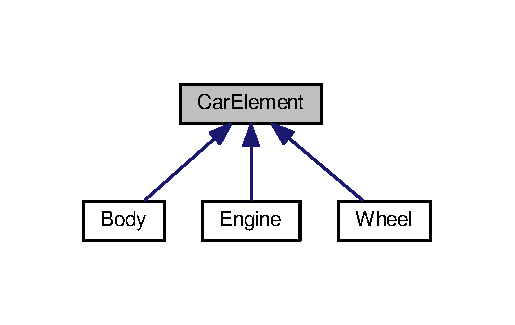
\includegraphics[width=247pt]{structCarElement__inherit__graph}
\end{center}
\end{figure}
\subsection*{Public Member Functions}
\begin{DoxyCompactItemize}
\item 
virtual void \hyperlink{structCarElement_a9cac92d2d59d9a0318600e608bbbdfd5}{accept} (const \hyperlink{structCarElementVisitor}{Car\+Element\+Visitor} \&visitor)=0
\item 
virtual \hyperlink{structCarElement_a320944d808655ea9ce077decb644518f}{$\sim$\+Car\+Element} ()
\end{DoxyCompactItemize}


\subsection{Constructor \& Destructor Documentation}
\index{Car\+Element@{Car\+Element}!````~Car\+Element@{$\sim$\+Car\+Element}}
\index{````~Car\+Element@{$\sim$\+Car\+Element}!Car\+Element@{Car\+Element}}
\subsubsection[{\texorpdfstring{$\sim$\+Car\+Element()}{~CarElement()}}]{\setlength{\rightskip}{0pt plus 5cm}virtual Car\+Element\+::$\sim$\+Car\+Element (
\begin{DoxyParamCaption}
{}
\end{DoxyParamCaption}
)\hspace{0.3cm}{\ttfamily [inline]}, {\ttfamily [virtual]}}\hypertarget{structCarElement_a320944d808655ea9ce077decb644518f}{}\label{structCarElement_a320944d808655ea9ce077decb644518f}

\begin{DoxyCode}
27 \{\}
\end{DoxyCode}


\subsection{Member Function Documentation}
\index{Car\+Element@{Car\+Element}!accept@{accept}}
\index{accept@{accept}!Car\+Element@{Car\+Element}}
\subsubsection[{\texorpdfstring{accept(const Car\+Element\+Visitor \&visitor)=0}{accept(const CarElementVisitor &visitor)=0}}]{\setlength{\rightskip}{0pt plus 5cm}virtual void Car\+Element\+::accept (
\begin{DoxyParamCaption}
\item[{const {\bf Car\+Element\+Visitor} \&}]{visitor}
\end{DoxyParamCaption}
)\hspace{0.3cm}{\ttfamily [pure virtual]}}\hypertarget{structCarElement_a9cac92d2d59d9a0318600e608bbbdfd5}{}\label{structCarElement_a9cac92d2d59d9a0318600e608bbbdfd5}


Implemented in \hyperlink{classBody_a1a00b0272b72001a9c40303b719de342}{Body}, \hyperlink{classEngine_ade04196721865cbebc12c0d34ad2a3d5}{Engine}, and \hyperlink{classWheel_acd6f77dbc8cea2223f5fd7810f4b80a6}{Wheel}.



The documentation for this struct was generated from the following file\+:\begin{DoxyCompactItemize}
\item 
\hyperlink{Visitor_8cpp}{Visitor.\+cpp}\end{DoxyCompactItemize}

\hypertarget{classCarElementDoVisitor}{}\section{Car\+Element\+Do\+Visitor Class Reference}
\label{classCarElementDoVisitor}\index{Car\+Element\+Do\+Visitor@{Car\+Element\+Do\+Visitor}}


Inheritance diagram for Car\+Element\+Do\+Visitor\+:
\nopagebreak
\begin{figure}[H]
\begin{center}
\leavevmode
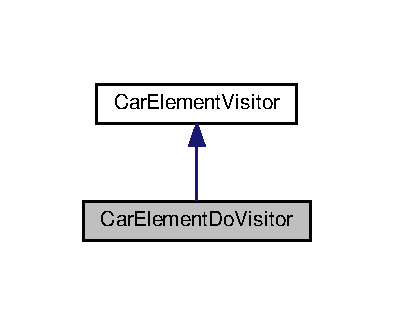
\includegraphics[width=189pt]{classCarElementDoVisitor__inherit__graph}
\end{center}
\end{figure}


Collaboration diagram for Car\+Element\+Do\+Visitor\+:
\nopagebreak
\begin{figure}[H]
\begin{center}
\leavevmode
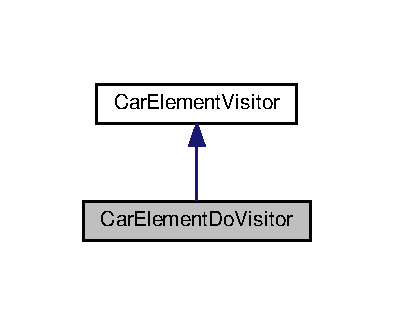
\includegraphics[width=189pt]{classCarElementDoVisitor__coll__graph}
\end{center}
\end{figure}
\subsection*{Public Member Functions}
\begin{DoxyCompactItemize}
\item 
void \hyperlink{classCarElementDoVisitor_a2c3ed0ee25fa1d7664d86dccb7d3d0d0}{visit} (\hyperlink{classWheel}{Wheel} \&wheel) const 
\item 
void \hyperlink{classCarElementDoVisitor_a51693652a685ca770761d5716ca752da}{visit} (\hyperlink{classEngine}{Engine} \&engine) const 
\item 
void \hyperlink{classCarElementDoVisitor_a5e3d87f05da1d9726d9518ff67993d96}{visit} (\hyperlink{classBody}{Body} \&body) const 
\item 
void \hyperlink{classCarElementDoVisitor_a067a72ca642eb15ebd11f975f9be2891}{visit\+Car} (\hyperlink{classCar}{Car} \&car) const 
\end{DoxyCompactItemize}


\subsection{Member Function Documentation}
\index{Car\+Element\+Do\+Visitor@{Car\+Element\+Do\+Visitor}!visit@{visit}}
\index{visit@{visit}!Car\+Element\+Do\+Visitor@{Car\+Element\+Do\+Visitor}}
\subsubsection[{\texorpdfstring{visit(\+Wheel \&wheel) const }{visit(Wheel &wheel) const }}]{\setlength{\rightskip}{0pt plus 5cm}void Car\+Element\+Do\+Visitor\+::visit (
\begin{DoxyParamCaption}
\item[{{\bf Wheel} \&}]{wheel}
\end{DoxyParamCaption}
) const\hspace{0.3cm}{\ttfamily [inline]}, {\ttfamily [virtual]}}\hypertarget{classCarElementDoVisitor_a2c3ed0ee25fa1d7664d86dccb7d3d0d0}{}\label{classCarElementDoVisitor_a2c3ed0ee25fa1d7664d86dccb7d3d0d0}


Implements \hyperlink{structCarElementVisitor_aba7f494a9b736bcb002176ec922890e4}{Car\+Element\+Visitor}.


\begin{DoxyCode}
135   \{
136     cout << \textcolor{stringliteral}{"Kicking my "} << wheel.\hyperlink{classWheel_ad0ed291d1ec488ffcba12e28cb707c38}{getName}() << \textcolor{stringliteral}{" wheel"} << endl;
137   \}
\end{DoxyCode}


Here is the call graph for this function\+:
\nopagebreak
\begin{figure}[H]
\begin{center}
\leavevmode
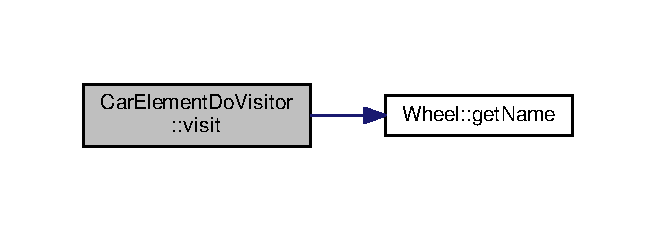
\includegraphics[width=315pt]{classCarElementDoVisitor_a2c3ed0ee25fa1d7664d86dccb7d3d0d0_cgraph}
\end{center}
\end{figure}


\index{Car\+Element\+Do\+Visitor@{Car\+Element\+Do\+Visitor}!visit@{visit}}
\index{visit@{visit}!Car\+Element\+Do\+Visitor@{Car\+Element\+Do\+Visitor}}
\subsubsection[{\texorpdfstring{visit(\+Engine \&engine) const }{visit(Engine &engine) const }}]{\setlength{\rightskip}{0pt plus 5cm}void Car\+Element\+Do\+Visitor\+::visit (
\begin{DoxyParamCaption}
\item[{{\bf Engine} \&}]{engine}
\end{DoxyParamCaption}
) const\hspace{0.3cm}{\ttfamily [inline]}, {\ttfamily [virtual]}}\hypertarget{classCarElementDoVisitor_a51693652a685ca770761d5716ca752da}{}\label{classCarElementDoVisitor_a51693652a685ca770761d5716ca752da}


Implements \hyperlink{structCarElementVisitor_aa0dabf5c22b4ebad04f01ec80f4c9eba}{Car\+Element\+Visitor}.


\begin{DoxyCode}
139   \{
140     cout << \textcolor{stringliteral}{"Starting my engine"} << endl;
141   \}
\end{DoxyCode}
\index{Car\+Element\+Do\+Visitor@{Car\+Element\+Do\+Visitor}!visit@{visit}}
\index{visit@{visit}!Car\+Element\+Do\+Visitor@{Car\+Element\+Do\+Visitor}}
\subsubsection[{\texorpdfstring{visit(\+Body \&body) const }{visit(Body &body) const }}]{\setlength{\rightskip}{0pt plus 5cm}void Car\+Element\+Do\+Visitor\+::visit (
\begin{DoxyParamCaption}
\item[{{\bf Body} \&}]{body}
\end{DoxyParamCaption}
) const\hspace{0.3cm}{\ttfamily [inline]}, {\ttfamily [virtual]}}\hypertarget{classCarElementDoVisitor_a5e3d87f05da1d9726d9518ff67993d96}{}\label{classCarElementDoVisitor_a5e3d87f05da1d9726d9518ff67993d96}


Implements \hyperlink{structCarElementVisitor_afc449830fe12235c3676039af8927fce}{Car\+Element\+Visitor}.


\begin{DoxyCode}
143   \{
144     cout << \textcolor{stringliteral}{"Moving my body"} << endl;
145   \}
\end{DoxyCode}
\index{Car\+Element\+Do\+Visitor@{Car\+Element\+Do\+Visitor}!visit\+Car@{visit\+Car}}
\index{visit\+Car@{visit\+Car}!Car\+Element\+Do\+Visitor@{Car\+Element\+Do\+Visitor}}
\subsubsection[{\texorpdfstring{visit\+Car(\+Car \&car) const }{visitCar(Car &car) const }}]{\setlength{\rightskip}{0pt plus 5cm}void Car\+Element\+Do\+Visitor\+::visit\+Car (
\begin{DoxyParamCaption}
\item[{{\bf Car} \&}]{car}
\end{DoxyParamCaption}
) const\hspace{0.3cm}{\ttfamily [inline]}, {\ttfamily [virtual]}}\hypertarget{classCarElementDoVisitor_a067a72ca642eb15ebd11f975f9be2891}{}\label{classCarElementDoVisitor_a067a72ca642eb15ebd11f975f9be2891}


Implements \hyperlink{structCarElementVisitor_a91746881206fd9dc9b10f9e2fdb5cf58}{Car\+Element\+Visitor}.


\begin{DoxyCode}
147   \{
148     cout << endl << \textcolor{stringliteral}{"Starting my car"} << endl;
149     vector<CarElement*>& elems = car.\hyperlink{classCar_a70d9577f631b92e0537ff331c8f7409b}{getElements}();
150     \textcolor{keywordflow}{for}(vector<CarElement*>::iterator it = elems.begin();
151       it != elems.end(); ++it )
152     \{
153       (*it)->accept(*\textcolor{keyword}{this}); \textcolor{comment}{// this issues the callback i.e. to this from the element  }
154     \}
155     cout << \textcolor{stringliteral}{"Stopped car"} << endl;
156   \}
\end{DoxyCode}


Here is the call graph for this function\+:
\nopagebreak
\begin{figure}[H]
\begin{center}
\leavevmode
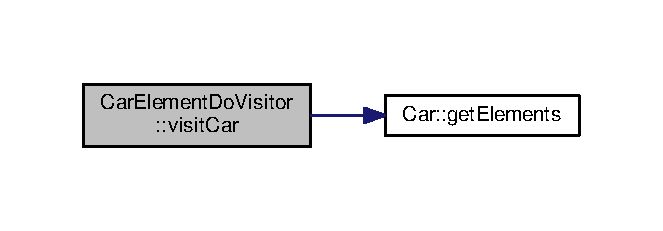
\includegraphics[width=318pt]{classCarElementDoVisitor_a067a72ca642eb15ebd11f975f9be2891_cgraph}
\end{center}
\end{figure}




The documentation for this class was generated from the following file\+:\begin{DoxyCompactItemize}
\item 
\hyperlink{Visitor_8cpp}{Visitor.\+cpp}\end{DoxyCompactItemize}

\hypertarget{classCarElementPrintVisitor}{}\section{Car\+Element\+Print\+Visitor Class Reference}
\label{classCarElementPrintVisitor}\index{Car\+Element\+Print\+Visitor@{Car\+Element\+Print\+Visitor}}


Inheritance diagram for Car\+Element\+Print\+Visitor\+:
\nopagebreak
\begin{figure}[H]
\begin{center}
\leavevmode
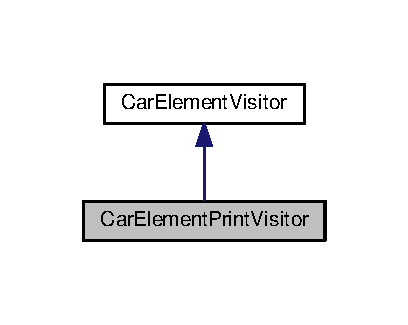
\includegraphics[width=196pt]{classCarElementPrintVisitor__inherit__graph}
\end{center}
\end{figure}


Collaboration diagram for Car\+Element\+Print\+Visitor\+:
\nopagebreak
\begin{figure}[H]
\begin{center}
\leavevmode
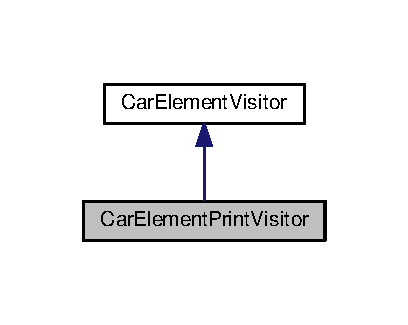
\includegraphics[width=196pt]{classCarElementPrintVisitor__coll__graph}
\end{center}
\end{figure}
\subsection*{Public Member Functions}
\begin{DoxyCompactItemize}
\item 
void \hyperlink{classCarElementPrintVisitor_a9677cd2f8d34aaf2a878ff1504e49c33}{visit} (\hyperlink{classWheel}{Wheel} \&wheel) const 
\item 
void \hyperlink{classCarElementPrintVisitor_afb71a1c5b2d6625bf569366f5903d531}{visit} (\hyperlink{classEngine}{Engine} \&engine) const 
\item 
void \hyperlink{classCarElementPrintVisitor_a4ad0bbfd79baaedfb2ee07c9e52d8f21}{visit} (\hyperlink{classBody}{Body} \&body) const 
\item 
void \hyperlink{classCarElementPrintVisitor_a99cb1306db917e1980d3f8c414acbc93}{visit\+Car} (\hyperlink{classCar}{Car} \&car) const 
\end{DoxyCompactItemize}


\subsection{Member Function Documentation}
\index{Car\+Element\+Print\+Visitor@{Car\+Element\+Print\+Visitor}!visit@{visit}}
\index{visit@{visit}!Car\+Element\+Print\+Visitor@{Car\+Element\+Print\+Visitor}}
\subsubsection[{\texorpdfstring{visit(\+Wheel \&wheel) const }{visit(Wheel &wheel) const }}]{\setlength{\rightskip}{0pt plus 5cm}void Car\+Element\+Print\+Visitor\+::visit (
\begin{DoxyParamCaption}
\item[{{\bf Wheel} \&}]{wheel}
\end{DoxyParamCaption}
) const\hspace{0.3cm}{\ttfamily [inline]}, {\ttfamily [virtual]}}\hypertarget{classCarElementPrintVisitor_a9677cd2f8d34aaf2a878ff1504e49c33}{}\label{classCarElementPrintVisitor_a9677cd2f8d34aaf2a878ff1504e49c33}


Implements \hyperlink{structCarElementVisitor_aba7f494a9b736bcb002176ec922890e4}{Car\+Element\+Visitor}.


\begin{DoxyCode}
106   \{ 
107     cout << \textcolor{stringliteral}{"Visiting "} << wheel.\hyperlink{classWheel_ad0ed291d1ec488ffcba12e28cb707c38}{getName}() << \textcolor{stringliteral}{" wheel"} << endl;
108   \}
\end{DoxyCode}


Here is the call graph for this function\+:
\nopagebreak
\begin{figure}[H]
\begin{center}
\leavevmode
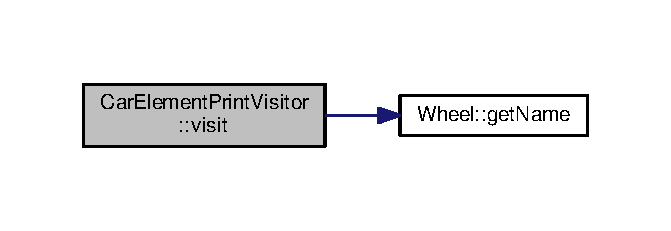
\includegraphics[width=322pt]{classCarElementPrintVisitor_a9677cd2f8d34aaf2a878ff1504e49c33_cgraph}
\end{center}
\end{figure}


\index{Car\+Element\+Print\+Visitor@{Car\+Element\+Print\+Visitor}!visit@{visit}}
\index{visit@{visit}!Car\+Element\+Print\+Visitor@{Car\+Element\+Print\+Visitor}}
\subsubsection[{\texorpdfstring{visit(\+Engine \&engine) const }{visit(Engine &engine) const }}]{\setlength{\rightskip}{0pt plus 5cm}void Car\+Element\+Print\+Visitor\+::visit (
\begin{DoxyParamCaption}
\item[{{\bf Engine} \&}]{engine}
\end{DoxyParamCaption}
) const\hspace{0.3cm}{\ttfamily [inline]}, {\ttfamily [virtual]}}\hypertarget{classCarElementPrintVisitor_afb71a1c5b2d6625bf569366f5903d531}{}\label{classCarElementPrintVisitor_afb71a1c5b2d6625bf569366f5903d531}


Implements \hyperlink{structCarElementVisitor_aa0dabf5c22b4ebad04f01ec80f4c9eba}{Car\+Element\+Visitor}.


\begin{DoxyCode}
110   \{
111     cout << \textcolor{stringliteral}{"Visiting engine"} << endl;
112   \}
\end{DoxyCode}
\index{Car\+Element\+Print\+Visitor@{Car\+Element\+Print\+Visitor}!visit@{visit}}
\index{visit@{visit}!Car\+Element\+Print\+Visitor@{Car\+Element\+Print\+Visitor}}
\subsubsection[{\texorpdfstring{visit(\+Body \&body) const }{visit(Body &body) const }}]{\setlength{\rightskip}{0pt plus 5cm}void Car\+Element\+Print\+Visitor\+::visit (
\begin{DoxyParamCaption}
\item[{{\bf Body} \&}]{body}
\end{DoxyParamCaption}
) const\hspace{0.3cm}{\ttfamily [inline]}, {\ttfamily [virtual]}}\hypertarget{classCarElementPrintVisitor_a4ad0bbfd79baaedfb2ee07c9e52d8f21}{}\label{classCarElementPrintVisitor_a4ad0bbfd79baaedfb2ee07c9e52d8f21}


Implements \hyperlink{structCarElementVisitor_afc449830fe12235c3676039af8927fce}{Car\+Element\+Visitor}.


\begin{DoxyCode}
114   \{
115     cout << \textcolor{stringliteral}{"Visiting body"} << endl;
116   \}
\end{DoxyCode}
\index{Car\+Element\+Print\+Visitor@{Car\+Element\+Print\+Visitor}!visit\+Car@{visit\+Car}}
\index{visit\+Car@{visit\+Car}!Car\+Element\+Print\+Visitor@{Car\+Element\+Print\+Visitor}}
\subsubsection[{\texorpdfstring{visit\+Car(\+Car \&car) const }{visitCar(Car &car) const }}]{\setlength{\rightskip}{0pt plus 5cm}void Car\+Element\+Print\+Visitor\+::visit\+Car (
\begin{DoxyParamCaption}
\item[{{\bf Car} \&}]{car}
\end{DoxyParamCaption}
) const\hspace{0.3cm}{\ttfamily [inline]}, {\ttfamily [virtual]}}\hypertarget{classCarElementPrintVisitor_a99cb1306db917e1980d3f8c414acbc93}{}\label{classCarElementPrintVisitor_a99cb1306db917e1980d3f8c414acbc93}


Implements \hyperlink{structCarElementVisitor_a91746881206fd9dc9b10f9e2fdb5cf58}{Car\+Element\+Visitor}.


\begin{DoxyCode}
118   \{
119     cout << endl << \textcolor{stringliteral}{"Visiting car"} << endl;
120     vector<CarElement*>& elems = car.\hyperlink{classCar_a70d9577f631b92e0537ff331c8f7409b}{getElements}();
121     \textcolor{keywordflow}{for}(vector<CarElement*>::iterator it = elems.begin();
122       it != elems.end(); ++it )
123     \{
124       (*it)->accept(*\textcolor{keyword}{this}); \textcolor{comment}{// this issues the callback i.e. to this from the element  }
125     \}
126     cout << \textcolor{stringliteral}{"Visited car"} << endl;
127   \}
\end{DoxyCode}


Here is the call graph for this function\+:
\nopagebreak
\begin{figure}[H]
\begin{center}
\leavevmode
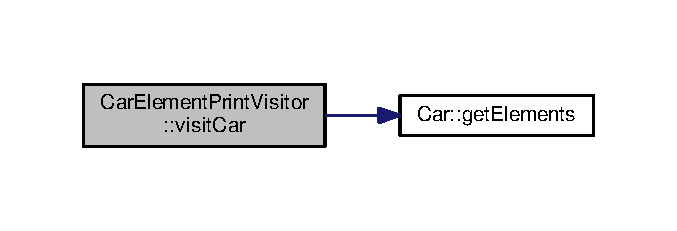
\includegraphics[width=325pt]{classCarElementPrintVisitor_a99cb1306db917e1980d3f8c414acbc93_cgraph}
\end{center}
\end{figure}




The documentation for this class was generated from the following file\+:\begin{DoxyCompactItemize}
\item 
\hyperlink{Visitor_8cpp}{Visitor.\+cpp}\end{DoxyCompactItemize}

\hypertarget{structCarElementVisitor}{}\section{Car\+Element\+Visitor Struct Reference}
\label{structCarElementVisitor}\index{Car\+Element\+Visitor@{Car\+Element\+Visitor}}


Inheritance diagram for Car\+Element\+Visitor\+:
\nopagebreak
\begin{figure}[H]
\begin{center}
\leavevmode
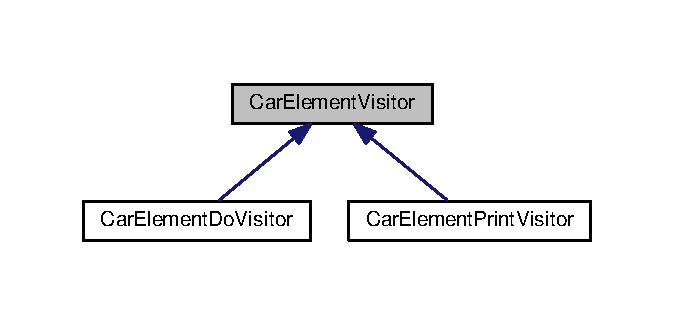
\includegraphics[width=324pt]{structCarElementVisitor__inherit__graph}
\end{center}
\end{figure}
\subsection*{Public Member Functions}
\begin{DoxyCompactItemize}
\item 
virtual void \hyperlink{structCarElementVisitor_aba7f494a9b736bcb002176ec922890e4}{visit} (\hyperlink{classWheel}{Wheel} \&wheel) const =0
\item 
virtual void \hyperlink{structCarElementVisitor_aa0dabf5c22b4ebad04f01ec80f4c9eba}{visit} (\hyperlink{classEngine}{Engine} \&engine) const =0
\item 
virtual void \hyperlink{structCarElementVisitor_afc449830fe12235c3676039af8927fce}{visit} (\hyperlink{classBody}{Body} \&body) const =0
\item 
virtual void \hyperlink{structCarElementVisitor_a91746881206fd9dc9b10f9e2fdb5cf58}{visit\+Car} (\hyperlink{classCar}{Car} \&car) const =0
\item 
virtual \hyperlink{structCarElementVisitor_aeb0329ef35c56ee6f84afa8471283391}{$\sim$\+Car\+Element\+Visitor} ()
\end{DoxyCompactItemize}


\subsection{Constructor \& Destructor Documentation}
\index{Car\+Element\+Visitor@{Car\+Element\+Visitor}!````~Car\+Element\+Visitor@{$\sim$\+Car\+Element\+Visitor}}
\index{````~Car\+Element\+Visitor@{$\sim$\+Car\+Element\+Visitor}!Car\+Element\+Visitor@{Car\+Element\+Visitor}}
\subsubsection[{\texorpdfstring{$\sim$\+Car\+Element\+Visitor()}{~CarElementVisitor()}}]{\setlength{\rightskip}{0pt plus 5cm}virtual Car\+Element\+Visitor\+::$\sim$\+Car\+Element\+Visitor (
\begin{DoxyParamCaption}
{}
\end{DoxyParamCaption}
)\hspace{0.3cm}{\ttfamily [inline]}, {\ttfamily [virtual]}}\hypertarget{structCarElementVisitor_aeb0329ef35c56ee6f84afa8471283391}{}\label{structCarElementVisitor_aeb0329ef35c56ee6f84afa8471283391}

\begin{DoxyCode}
20 \{\};
\end{DoxyCode}


\subsection{Member Function Documentation}
\index{Car\+Element\+Visitor@{Car\+Element\+Visitor}!visit@{visit}}
\index{visit@{visit}!Car\+Element\+Visitor@{Car\+Element\+Visitor}}
\subsubsection[{\texorpdfstring{visit(\+Wheel \&wheel) const =0}{visit(Wheel &wheel) const =0}}]{\setlength{\rightskip}{0pt plus 5cm}virtual void Car\+Element\+Visitor\+::visit (
\begin{DoxyParamCaption}
\item[{{\bf Wheel} \&}]{wheel}
\end{DoxyParamCaption}
) const\hspace{0.3cm}{\ttfamily [pure virtual]}}\hypertarget{structCarElementVisitor_aba7f494a9b736bcb002176ec922890e4}{}\label{structCarElementVisitor_aba7f494a9b736bcb002176ec922890e4}


Implemented in \hyperlink{classCarElementDoVisitor_a2c3ed0ee25fa1d7664d86dccb7d3d0d0}{Car\+Element\+Do\+Visitor}, and \hyperlink{classCarElementPrintVisitor_a9677cd2f8d34aaf2a878ff1504e49c33}{Car\+Element\+Print\+Visitor}.

\index{Car\+Element\+Visitor@{Car\+Element\+Visitor}!visit@{visit}}
\index{visit@{visit}!Car\+Element\+Visitor@{Car\+Element\+Visitor}}
\subsubsection[{\texorpdfstring{visit(\+Engine \&engine) const =0}{visit(Engine &engine) const =0}}]{\setlength{\rightskip}{0pt plus 5cm}virtual void Car\+Element\+Visitor\+::visit (
\begin{DoxyParamCaption}
\item[{{\bf Engine} \&}]{engine}
\end{DoxyParamCaption}
) const\hspace{0.3cm}{\ttfamily [pure virtual]}}\hypertarget{structCarElementVisitor_aa0dabf5c22b4ebad04f01ec80f4c9eba}{}\label{structCarElementVisitor_aa0dabf5c22b4ebad04f01ec80f4c9eba}


Implemented in \hyperlink{classCarElementDoVisitor_a51693652a685ca770761d5716ca752da}{Car\+Element\+Do\+Visitor}, and \hyperlink{classCarElementPrintVisitor_afb71a1c5b2d6625bf569366f5903d531}{Car\+Element\+Print\+Visitor}.

\index{Car\+Element\+Visitor@{Car\+Element\+Visitor}!visit@{visit}}
\index{visit@{visit}!Car\+Element\+Visitor@{Car\+Element\+Visitor}}
\subsubsection[{\texorpdfstring{visit(\+Body \&body) const =0}{visit(Body &body) const =0}}]{\setlength{\rightskip}{0pt plus 5cm}virtual void Car\+Element\+Visitor\+::visit (
\begin{DoxyParamCaption}
\item[{{\bf Body} \&}]{body}
\end{DoxyParamCaption}
) const\hspace{0.3cm}{\ttfamily [pure virtual]}}\hypertarget{structCarElementVisitor_afc449830fe12235c3676039af8927fce}{}\label{structCarElementVisitor_afc449830fe12235c3676039af8927fce}


Implemented in \hyperlink{classCarElementDoVisitor_a5e3d87f05da1d9726d9518ff67993d96}{Car\+Element\+Do\+Visitor}, and \hyperlink{classCarElementPrintVisitor_a4ad0bbfd79baaedfb2ee07c9e52d8f21}{Car\+Element\+Print\+Visitor}.

\index{Car\+Element\+Visitor@{Car\+Element\+Visitor}!visit\+Car@{visit\+Car}}
\index{visit\+Car@{visit\+Car}!Car\+Element\+Visitor@{Car\+Element\+Visitor}}
\subsubsection[{\texorpdfstring{visit\+Car(\+Car \&car) const =0}{visitCar(Car &car) const =0}}]{\setlength{\rightskip}{0pt plus 5cm}virtual void Car\+Element\+Visitor\+::visit\+Car (
\begin{DoxyParamCaption}
\item[{{\bf Car} \&}]{car}
\end{DoxyParamCaption}
) const\hspace{0.3cm}{\ttfamily [pure virtual]}}\hypertarget{structCarElementVisitor_a91746881206fd9dc9b10f9e2fdb5cf58}{}\label{structCarElementVisitor_a91746881206fd9dc9b10f9e2fdb5cf58}


Implemented in \hyperlink{classCarElementDoVisitor_a067a72ca642eb15ebd11f975f9be2891}{Car\+Element\+Do\+Visitor}, and \hyperlink{classCarElementPrintVisitor_a99cb1306db917e1980d3f8c414acbc93}{Car\+Element\+Print\+Visitor}.



The documentation for this struct was generated from the following file\+:\begin{DoxyCompactItemize}
\item 
\hyperlink{Visitor_8cpp}{Visitor.\+cpp}\end{DoxyCompactItemize}

\hypertarget{classEngine}{}\section{Engine Class Reference}
\label{classEngine}\index{Engine@{Engine}}


Inheritance diagram for Engine\+:
\nopagebreak
\begin{figure}[H]
\begin{center}
\leavevmode
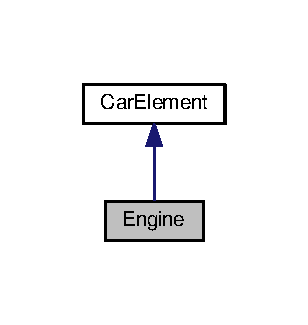
\includegraphics[width=148pt]{classEngine__inherit__graph}
\end{center}
\end{figure}


Collaboration diagram for Engine\+:
\nopagebreak
\begin{figure}[H]
\begin{center}
\leavevmode
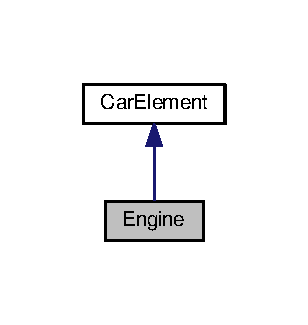
\includegraphics[width=148pt]{classEngine__coll__graph}
\end{center}
\end{figure}
\subsection*{Public Member Functions}
\begin{DoxyCompactItemize}
\item 
void \hyperlink{classEngine_ade04196721865cbebc12c0d34ad2a3d5}{accept} (const \hyperlink{structCarElementVisitor}{Car\+Element\+Visitor} \&visitor)
\end{DoxyCompactItemize}


\subsection{Member Function Documentation}
\index{Engine@{Engine}!accept@{accept}}
\index{accept@{accept}!Engine@{Engine}}
\subsubsection[{\texorpdfstring{accept(const Car\+Element\+Visitor \&visitor)}{accept(const CarElementVisitor &visitor)}}]{\setlength{\rightskip}{0pt plus 5cm}void Engine\+::accept (
\begin{DoxyParamCaption}
\item[{const {\bf Car\+Element\+Visitor} \&}]{visitor}
\end{DoxyParamCaption}
)\hspace{0.3cm}{\ttfamily [inline]}, {\ttfamily [virtual]}}\hypertarget{classEngine_ade04196721865cbebc12c0d34ad2a3d5}{}\label{classEngine_ade04196721865cbebc12c0d34ad2a3d5}


Implements \hyperlink{structCarElement_a9cac92d2d59d9a0318600e608bbbdfd5}{Car\+Element}.


\begin{DoxyCode}
55   \{
56     visitor.\hyperlink{structCarElementVisitor_aba7f494a9b736bcb002176ec922890e4}{visit}(*\textcolor{keyword}{this});
57   \}
\end{DoxyCode}


Here is the call graph for this function\+:
\nopagebreak
\begin{figure}[H]
\begin{center}
\leavevmode
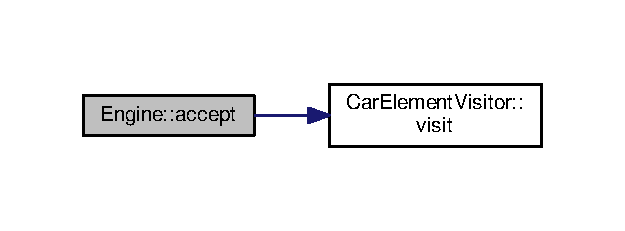
\includegraphics[width=300pt]{classEngine_ade04196721865cbebc12c0d34ad2a3d5_cgraph}
\end{center}
\end{figure}




The documentation for this class was generated from the following file\+:\begin{DoxyCompactItemize}
\item 
\hyperlink{Visitor_8cpp}{Visitor.\+cpp}\end{DoxyCompactItemize}

\hypertarget{classWheel}{}\section{Wheel Class Reference}
\label{classWheel}\index{Wheel@{Wheel}}


Inheritance diagram for Wheel\+:
\nopagebreak
\begin{figure}[H]
\begin{center}
\leavevmode
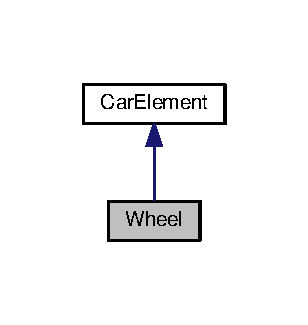
\includegraphics[width=148pt]{classWheel__inherit__graph}
\end{center}
\end{figure}


Collaboration diagram for Wheel\+:
\nopagebreak
\begin{figure}[H]
\begin{center}
\leavevmode
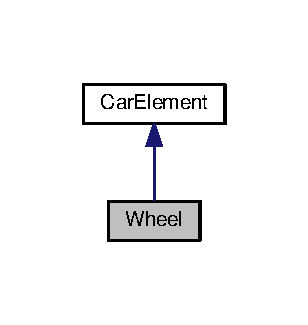
\includegraphics[width=148pt]{classWheel__coll__graph}
\end{center}
\end{figure}
\subsection*{Public Member Functions}
\begin{DoxyCompactItemize}
\item 
\hyperlink{classWheel_aa56122040fc03dbf3036fd649f749163}{Wheel} (const string \&name)
\item 
const string \& \hyperlink{classWheel_ad0ed291d1ec488ffcba12e28cb707c38}{get\+Name} () const 
\item 
void \hyperlink{classWheel_acd6f77dbc8cea2223f5fd7810f4b80a6}{accept} (const \hyperlink{structCarElementVisitor}{Car\+Element\+Visitor} \&visitor)
\end{DoxyCompactItemize}
\subsection*{Private Attributes}
\begin{DoxyCompactItemize}
\item 
string \hyperlink{classWheel_a2aff80b65a1531a7289349af36f15f3f}{name\+\_\+}
\end{DoxyCompactItemize}


\subsection{Constructor \& Destructor Documentation}
\index{Wheel@{Wheel}!Wheel@{Wheel}}
\index{Wheel@{Wheel}!Wheel@{Wheel}}
\subsubsection[{\texorpdfstring{Wheel(const string \&name)}{Wheel(const string &name)}}]{\setlength{\rightskip}{0pt plus 5cm}Wheel\+::\+Wheel (
\begin{DoxyParamCaption}
\item[{const string \&}]{name}
\end{DoxyParamCaption}
)\hspace{0.3cm}{\ttfamily [inline]}, {\ttfamily [explicit]}}\hypertarget{classWheel_aa56122040fc03dbf3036fd649f749163}{}\label{classWheel_aa56122040fc03dbf3036fd649f749163}

\begin{DoxyCode}
34                                      :
35     \hyperlink{classWheel_a2aff80b65a1531a7289349af36f15f3f}{name\_}(name)
36   \{
37   \}
\end{DoxyCode}


\subsection{Member Function Documentation}
\index{Wheel@{Wheel}!accept@{accept}}
\index{accept@{accept}!Wheel@{Wheel}}
\subsubsection[{\texorpdfstring{accept(const Car\+Element\+Visitor \&visitor)}{accept(const CarElementVisitor &visitor)}}]{\setlength{\rightskip}{0pt plus 5cm}void Wheel\+::accept (
\begin{DoxyParamCaption}
\item[{const {\bf Car\+Element\+Visitor} \&}]{visitor}
\end{DoxyParamCaption}
)\hspace{0.3cm}{\ttfamily [inline]}, {\ttfamily [virtual]}}\hypertarget{classWheel_acd6f77dbc8cea2223f5fd7810f4b80a6}{}\label{classWheel_acd6f77dbc8cea2223f5fd7810f4b80a6}


Implements \hyperlink{structCarElement_a9cac92d2d59d9a0318600e608bbbdfd5}{Car\+Element}.


\begin{DoxyCode}
43   \{
44     visitor.\hyperlink{structCarElementVisitor_aba7f494a9b736bcb002176ec922890e4}{visit}(*\textcolor{keyword}{this});
45   \}
\end{DoxyCode}


Here is the call graph for this function\+:
\nopagebreak
\begin{figure}[H]
\begin{center}
\leavevmode
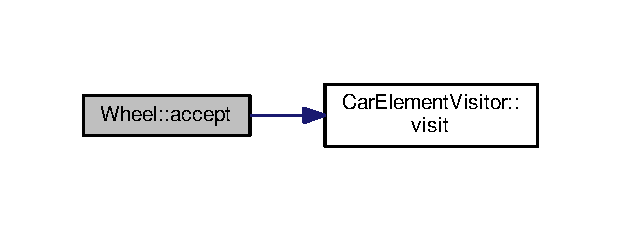
\includegraphics[width=298pt]{classWheel_acd6f77dbc8cea2223f5fd7810f4b80a6_cgraph}
\end{center}
\end{figure}


\index{Wheel@{Wheel}!get\+Name@{get\+Name}}
\index{get\+Name@{get\+Name}!Wheel@{Wheel}}
\subsubsection[{\texorpdfstring{get\+Name() const }{getName() const }}]{\setlength{\rightskip}{0pt plus 5cm}const string\& Wheel\+::get\+Name (
\begin{DoxyParamCaption}
{}
\end{DoxyParamCaption}
) const\hspace{0.3cm}{\ttfamily [inline]}}\hypertarget{classWheel_ad0ed291d1ec488ffcba12e28cb707c38}{}\label{classWheel_ad0ed291d1ec488ffcba12e28cb707c38}

\begin{DoxyCode}
39   \{
40     \textcolor{keywordflow}{return} \hyperlink{classWheel_a2aff80b65a1531a7289349af36f15f3f}{name\_};
41   \}
\end{DoxyCode}


\subsection{Member Data Documentation}
\index{Wheel@{Wheel}!name\+\_\+@{name\+\_\+}}
\index{name\+\_\+@{name\+\_\+}!Wheel@{Wheel}}
\subsubsection[{\texorpdfstring{name\+\_\+}{name_}}]{\setlength{\rightskip}{0pt plus 5cm}string Wheel\+::name\+\_\+\hspace{0.3cm}{\ttfamily [private]}}\hypertarget{classWheel_a2aff80b65a1531a7289349af36f15f3f}{}\label{classWheel_a2aff80b65a1531a7289349af36f15f3f}


The documentation for this class was generated from the following file\+:\begin{DoxyCompactItemize}
\item 
\hyperlink{Visitor_8cpp}{Visitor.\+cpp}\end{DoxyCompactItemize}

\chapter{File Documentation}
\hypertarget{Visitor_8cpp}{}\section{Visitor.\+cpp File Reference}
\label{Visitor_8cpp}\index{Visitor.\+cpp@{Visitor.\+cpp}}
{\ttfamily \#include $<$string$>$}\\*
{\ttfamily \#include $<$iostream$>$}\\*
{\ttfamily \#include $<$vector$>$}\\*
Include dependency graph for Visitor.\+cpp\+:
\nopagebreak
\begin{figure}[H]
\begin{center}
\leavevmode
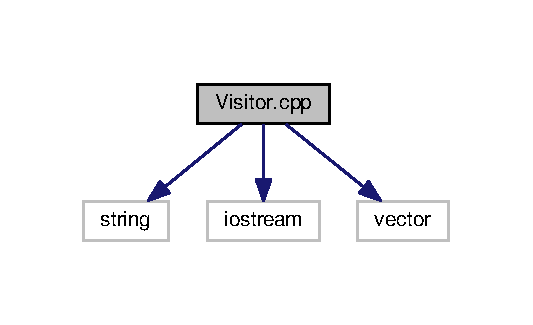
\includegraphics[width=256pt]{Visitor_8cpp__incl}
\end{center}
\end{figure}
\subsection*{Classes}
\begin{DoxyCompactItemize}
\item 
struct \hyperlink{structCarElementVisitor}{Car\+Element\+Visitor}
\item 
struct \hyperlink{structCarElement}{Car\+Element}
\item 
class \hyperlink{classWheel}{Wheel}
\item 
class \hyperlink{classEngine}{Engine}
\item 
class \hyperlink{classBody}{Body}
\item 
class \hyperlink{classCar}{Car}
\item 
class \hyperlink{classCarElementPrintVisitor}{Car\+Element\+Print\+Visitor}
\item 
class \hyperlink{classCarElementDoVisitor}{Car\+Element\+Do\+Visitor}
\end{DoxyCompactItemize}
\subsection*{Functions}
\begin{DoxyCompactItemize}
\item 
int \hyperlink{Visitor_8cpp_ae66f6b31b5ad750f1fe042a706a4e3d4}{main} ()
\end{DoxyCompactItemize}


\subsection{Function Documentation}
\index{Visitor.\+cpp@{Visitor.\+cpp}!main@{main}}
\index{main@{main}!Visitor.\+cpp@{Visitor.\+cpp}}
\subsubsection[{\texorpdfstring{main()}{main()}}]{\setlength{\rightskip}{0pt plus 5cm}int main (
\begin{DoxyParamCaption}
{}
\end{DoxyParamCaption}
)}\hypertarget{Visitor_8cpp_ae66f6b31b5ad750f1fe042a706a4e3d4}{}\label{Visitor_8cpp_ae66f6b31b5ad750f1fe042a706a4e3d4}

\begin{DoxyCode}
160 \{
161   \hyperlink{classCar}{Car} car;
162   \hyperlink{classCarElementPrintVisitor}{CarElementPrintVisitor} printVisitor;
163   \hyperlink{classCarElementDoVisitor}{CarElementDoVisitor} doVisitor;
164   
165   printVisitor.\hyperlink{classCarElementPrintVisitor_a99cb1306db917e1980d3f8c414acbc93}{visitCar}(car);
166   doVisitor.\hyperlink{classCarElementDoVisitor_a067a72ca642eb15ebd11f975f9be2891}{visitCar}(car);
167 
168   \textcolor{keywordflow}{return} 0;
169 \}\end{DoxyCode}


Here is the call graph for this function\+:
\nopagebreak
\begin{figure}[H]
\begin{center}
\leavevmode
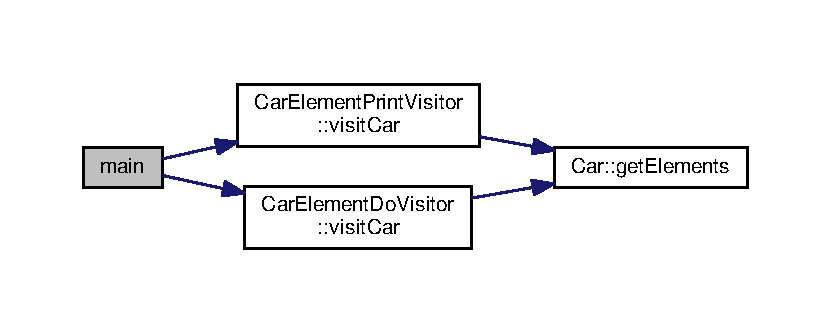
\includegraphics[width=350pt]{Visitor_8cpp_ae66f6b31b5ad750f1fe042a706a4e3d4_cgraph}
\end{center}
\end{figure}



%--- End generated contents ---

% Index
\backmatter
\newpage
\phantomsection
\clearemptydoublepage
\addcontentsline{toc}{chapter}{Index}
\printindex

\end{document}
